\section{Endpoint bounds}\label{sec:endpoint}

This section proves Theorems A, B and C. The two results we cite, the sparse domination theorem
of Beltran, Roos and Seeger and the weighted theorem of Frey and Nieraeth, are stated first in the
form in which they are used. Throughout, $R^\lambda_a=R^\lambda_{a,1}$.

\subsection{Sparse forms}\label{ssec:sparse}
A \emph{dyadic lattice} in the sense of \cite[\S2]{LN19} is a family $\D$ of cubes in $\R^n$ such
that the $2^n$ halves of every cube of $\D$ belong to $\D$, every two cubes of $\D$ are contained in a
common cube of $\D$, and every compact set is contained in a cube of $\D$. For a cube $Q$, a locally
integrable $f$ and $1\le p<\infty$ put $\langle f\rangle_{Q,p}=\bigl(|Q|^{-1}\int_Q|f|^p\bigr)^{1/p}$.

\begin{definition}\label{def:sparse}
Let $0<\gamma<1$. A family $\mathcal S$ of cubes, each belonging to some dyadic lattice, is
\emph{$\gamma$-sparse} if there are pairwise disjoint measurable sets $E_Q\subset Q$, $Q\in\mathcal S$,
with $|E_Q|\ge\gamma|Q|$. For $1\le p,q<\infty$ put
\[
\Lambda^{\mathcal S}_{p,q}(f_1,f_2)=\sum_{Q\in\mathcal S}|Q|\,\langle f_1\rangle_{Q,p}\langle f_2\rangle_{Q,q},
\qquad
\Lambda^*_{p,q}(f_1,f_2)=\sup_{\mathcal S}\Lambda^{\mathcal S}_{p,q}(f_1,f_2),
\]
the supremum over all $\gamma$-sparse families. A linear operator $T$ from $C^\infty_c(\R^n)$ to
distributions belongs to $\Sp(p,q)$ if there is $C$ with
\begin{equation}\label{eq:sparse}
|\ip{Tf_1}{f_2}|\le C\,\Lambda^*_{p,q}(f_1,f_2)\qquad(f_1,f_2\in C^\infty_c(\R^n)),
\end{equation}
and $\|T\|_{\Sp(p,q)}$ is the least such $C$.
\end{definition}

Here $\ip{f}{g}=\int fg$. This is \cite[(1.2)--(1.4)]{BRS25}. The class $\Sp(p,q)$ does not depend on
$\gamma$ \cite{LN19}, and we fix $\gamma=\frac12$. Since $\langle f\rangle_{Q,p}$ increases with $p$,
$\Sp(p,q)\subset\Sp(\tilde p,\tilde q)$ when $p\le\tilde p$ and $q\le\tilde q$.

\begin{lemma}\label{lem:dilation}
Let $T$ be a Fourier multiplier operator $m(D)$ with $m\in L^\infty$, and $T_t=m(D/t)$ for $t>0$.
Then $\|T_t\|_{\Sp(p,q)}=\|T\|_{\Sp(p,q)}$.
\end{lemma}

\begin{proof}
For $f\in C^\infty_c$ put $f^{(t)}(y)=f(y/t)$. Its Fourier transform is $t^n\hat f(t\xi)$, so
\[
T(f^{(t)})(y)=\frac1{(2\pi)^n}\int m(\xi)\,t^n\hat f(t\xi)e^{i\ip y\xi}\,d\xi
=\frac1{(2\pi)^n}\int m(\eta/t)\hat f(\eta)e^{i\ip{y/t}{\eta}}\,d\eta=T_tf(y/t).
\]
Hence $\ip{T_tf_1}{f_2}=\int T(f_1^{(t)})(tx)f_2(x)\,dx=t^{-n}\ip{Tf_1^{(t)}}{f_2^{(t)}}$. For a cube $Q$,
$\langle f^{(t)}\rangle_{Q,p}=\langle f\rangle_{t^{-1}Q,p}$ and $|Q|=t^n|t^{-1}Q|$. The image of a dyadic
lattice under $x\mapsto t^{-1}x$ is a dyadic lattice, and the image of a $\gamma$-sparse family is
$\gamma$-sparse, with the sets $t^{-1}E_Q$. Therefore
$t^{-n}\Lambda^{\mathcal S}_{p,q}(f_1^{(t)},f_2^{(t)})=\Lambda^{t^{-1}\mathcal S}_{p,q}(f_1,f_2)\le\Lambda^*_{p,q}(f_1,f_2)$,
and $\|T_t\|_{\Sp(p,q)}\le\|T\|_{\Sp(p,q)}$. Exchanging the roles of $T$ and $T_t$ gives equality.
\end{proof}

\subsection{The sparse domination theorem}\label{ssec:brs}
For $1\le p<p_\circ<\frac{2n}{n+1}$ with $p_{\rm ST}\le p_\circ$ define $q_*(p,p_\circ)$ by
\begin{equation}\label{eq:qstar}
1-\frac1{q_*(p,p_\circ)}=
\begin{cases}
\dfrac1{r_*(p,p_\circ)}&\text{if }p_{\rm ST}\le p<p_\circ,\\[2mm]
\dfrac{n+1}{n-1}\Bigl(1-\dfrac1p\Bigr)&\text{if }1\le p\le p_{\rm ST},
\end{cases}
\end{equation}
with $r_*$ from \eqref{eq:rstar}. Both lines give $\frac12$ at $p=p_{\rm ST}$, since
$\frac{n+1}{n-1}(1-\frac{n+3}{2(n+1)})=\frac12$. This is \cite[(2.1)]{BRS25} with $r_\circ=p_\circ$: the
first line of \cite[(2.1)]{BRS25} has weights $\frac1{r_\circ}$ and $\frac12$ on the same two
differences as \eqref{eq:rstar}. For $p\le p_{\rm ST}$ the second line gives
\begin{equation}\label{eq:qopt}
q_*(p,p_\circ)=q_{\rm opt}(p)=\frac{(n-1)p}{n+1-2p},
\end{equation}
because $1-\frac{n+1-2p}{(n-1)p}=\frac{(n+1)(p-1)}{(n-1)p}$. The same computation and
\eqref{eq:rstarlimit} show that for $p_{\rm ST}\le p<\frac{2n}{n+1}$,
\begin{equation}\label{eq:qstarlimit}
\lim_{p_\circ\to\frac{2n}{n+1}}\Bigl(1-\frac1{q_*(p,p_\circ)}\Bigr)=\frac{n+1}{n-1}\Bigl(1-\frac1p\Bigr)
=1-\frac1{q_{\rm opt}(p)} .
\end{equation}

\begin{theorem}[{\cite[Theorem 2.3]{BRS25}}]\label{thm:brs}
Let $n\ge2$, $a>0$, $p_{\rm ST}\le p_\circ<\frac{2n}{n+1}$, and $p_\circ\le r_\circ\le\frac{n-1}{n+1}p_\circ'$.
Suppose that $\VBR(p,r)$ holds for all $p\in[p_{\rm ST},p_\circ)$ and $r\in[p,r_*(p,p_\circ,r_\circ))$. Then
$R^{\lambda(p)}_a\in\Sp(p,q)$ for $1\le p<p_\circ$ and $q>q_*(p,p_\circ,r_\circ)$.
\end{theorem}

In \cite{BRS25} the exponents $r_*(p,p_\circ,r_\circ)$, $q_*(p,p_\circ,r_\circ)$ are defined for every admissible
$r_\circ$, and $\VBR(p,r)$ is \cite[Definition 2.2]{BRS25}, which is Definition \ref{def:vbr} for the
Euclidean norm. We use only $r_\circ=p_\circ$, for which these exponents are $r_*(p,p_\circ)$ and
$q_*(p,p_\circ)$ above. The constraint $r_\circ\le\frac{n-1}{n+1}p_\circ'$ then reads
$p_\circ-1\le\frac{n-1}{n+1}$, that is $p_\circ\le\frac{2n}{n+1}$, which holds.

\subsection{Proof of Theorem B}\label{ssec:proofB}
Figure \ref{fig:sparse} shows the exponents reached for $n=3$.
Let $1\le p<\frac{2n}{n+1}$ and $q>q_{\rm opt}(p)$. By \eqref{eq:qopt} and \eqref{eq:qstarlimit} there
is $p_\circ$ with
\[
\max\{p,p_{\rm ST}\}<p_\circ<\tfrac{2n}{n+1},\qquad q>q_*(p,p_\circ):
\]
when $p\le p_{\rm ST}$ every $p_\circ\in(p_{\rm ST},\frac{2n}{n+1})$ will do, since then
$q_*(p,p_\circ)=q_{\rm opt}(p)$; when $p>p_{\rm ST}$, $1-\frac1{q_*}$ tends to $1-\frac1{q_{\rm opt}}<1-\frac1q$
as $p_\circ\to\frac{2n}{n+1}$. By Corollary \ref{cor:vbr}, $\VBR(\tilde p,r)$ holds for
$\tilde p\in[p_{\rm ST},p_\circ)$ and $r\in[\tilde p,r_*(\tilde p,p_\circ))$, which is the hypothesis of
Theorem \ref{thm:brs} with $r_\circ=p_\circ$. Hence $R^{\lambda(p)}_a\in\Sp(p,q)$. Since
$R^{\lambda(p)}_{a,t}=m(D/t)$ with $m(\xi)=(1-|\xi|^a)^{\lambda(p)}_+$, Lemma \ref{lem:dilation} gives
$\|R^{\lambda(p)}_{a,t}\|_{\Sp(p,q)}=\|R^{\lambda(p)}_a\|_{\Sp(p,q)}$ for every $t>0$. \qed

\begin{figure}[t]
\centering
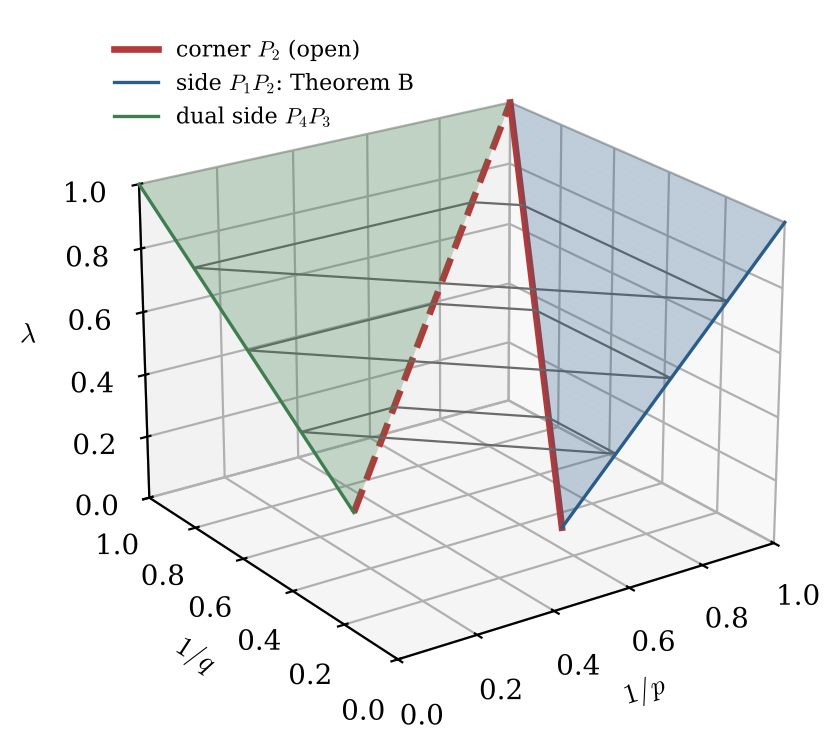
\includegraphics[width=0.78\textwidth]{figures/fig_sparse.png}
\caption{Sparse exponents $(1/p,1/q)$ for $n=3$ at height $\lambda=\lambda(p)$. The grey quadrilaterals
are the trapezoids $P_1P_2P_3P_4$ of \cite[(1.5)]{BRS25} at $\lambda=\frac14,\frac12,\frac34$. As
$\lambda$ runs over $(0,\frac{n-1}2)$ the critical side $P_1P_2$ sweeps the blue surface, which
Theorem B covers except for the red edge traced by the corner $P_2$, where $q=q_{\rm opt}(p)$; the
green surface and the dashed edge are their duals $P_4P_3$ and $P_3$.}
\label{fig:sparse}
\end{figure}

\subsection{Weights}\label{sec:weights}
A \emph{weight} is a locally integrable function $w>0$ almost everywhere. For a ball $B$ write
$\fint_Bw=|B|^{-1}\int_Bw$ and $w(E)=\int_Ew$. The weight belongs to $A_1$ if
\[
[w]_{A_1}=\sup_B\Bigl(\fint_Bw\Bigr)\Bigl(\operatorname*{ess\,inf}_Bw\Bigr)^{-1}<\infty,
\]
and, for $1<\sigma<\infty$, to $RH_\sigma$ if
\[
[w]_{RH_\sigma}=\sup_B\Bigl(\fint_Bw^\sigma\Bigr)^{1/\sigma}\Bigl(\fint_Bw\Bigr)^{-1}<\infty ,
\]
the suprema over all balls. By H\"older's inequality $RH_\sigma\subset RH_{\tilde\sigma}$ when
$\tilde\sigma<\sigma$. Every $A_1$ weight belongs to $RH_\sigma$ for some $\sigma>1$, by the reverse H\"older
inequality of Coifman and Fefferman \cite{CF74}, and $A_1\subset A_p$ for $p>1$, so the
Hardy--Littlewood maximal operator $M$ is bounded on $L^p(w)$ for $w\in A_1$ and $1<p<\infty$
\cite[Ch.~7]{Gra14}. The weak space $L^{p,\infty}(w)$ has the quasinorm
$\|f\|_{L^{p,\infty}(w)}=\sup_{s>0}s\,w(\{|f|>s\})^{1/p}$, which satisfies
$\|f+g\|_{L^{p,\infty}(w)}\le2(\|f\|_{L^{p,\infty}(w)}+\|g\|_{L^{p,\infty}(w)})$ and
$\|f\|_{L^{p,\infty}(w)}\le\|f\|_{L^p(w)}$, and $L^{p,\infty}(w)$ is complete.

\begin{theorem}[{\cite[Theorem 1.4]{FN19}}]\label{thm:fn}
Let $1\le p<q'$, so that $\frac1p+\frac1q>1$, and put $\sigma=(q'/p)'=\frac q{q+p-pq}$. There is a
function $\Phi$, increasing in each variable, such that every $T\in\Sp(p,q)$ satisfies
\[
\|Tf\|_{L^{p,\infty}(w)}\le\Phi\bigl([w]_{A_1},[w]_{RH_\sigma}\bigr)\,\|T\|_{\Sp(p,q)}\|f\|_{L^p(w)}
\qquad(f\in C^\infty_c(\R^n))
\]
for every $w\in A_1\cap RH_\sigma$.
\end{theorem}

This is \cite[Theorem 1.4]{FN19} in the notation of \cite[(9.2)]{BRS25}, where the constant is,
up to a factor depending on $n,p,q$,
\[
\|T\|_{\Sp(p,q)}[w^\sigma]_{A_\infty}^{1/p}[w]_{A_1}^{1+1/p}[w]_{RH_\sigma}^{1/p},
\]
and $[v]_{A_\infty}=\sup_Bv(B)^{-1}\int_BM(v\mathbf 1_B)$ is Wilson's constant. It is bounded by
a function of $[w]_{A_1}$ and $[w]_{RH_\sigma}$: for every ball,
\[
\fint_Bw^\sigma\le[w]_{RH_\sigma}^\sigma\Bigl(\fint_Bw\Bigr)^\sigma\le([w]_{RH_\sigma}[w]_{A_1})^\sigma
\operatorname*{ess\,inf}_Bw^\sigma ,
\]
so $v=w^\sigma\in A_1$ with $[v]_{A_1}\le([w]_{RH_\sigma}[w]_{A_1})^\sigma$; then $Mv\le[v]_{A_1}v$ almost
everywhere, for $M$ the maximal operator over balls containing the point, and
$[v]_{A_\infty}\le[v]_{A_1}$.

\subsection{Proof of Theorem C}\label{ssec:proofC}
Let $w\in A_1\cap RH_\sigma$ with $\sigma>1$, and $1<p<p_1(w)=1+\frac{n-1}{n+1}(1-\frac1\sigma)$. Then
$p<\frac{2n}{n+1}$. For $q\in(q_{\rm opt}(p),p')$ put $\sigma(q)=\frac q{q+p-pq}$, the exponent of Theorem
\ref{thm:fn}. The interval is not empty: $q_{\rm opt}(p)<p'$ is equivalent to
$(n-1)(p-1)<n+1-2p$, that is to $p<\frac{2n}{n+1}$. On it the denominator
$q+p-pq=q\bigl(1-p(1-\frac1q)\bigr)$ is positive, since $1-\frac1q<\frac1p$, and
$\sigma(q)=\bigl(1+\frac pq-p\bigr)^{-1}$ is continuous and increasing in $q$. At $q=q_{\rm opt}(p)$,
\[
q+p-pq=\frac{(n-1)p(1-p)+p(n+1-2p)}{n+1-2p}=\frac{p\,(2n-(n+1)p)}{n+1-2p},
\]
so that
\[
\sigma(q_{\rm opt}(p))=\frac{n-1}{2n-(n+1)p} .
\]
The hypothesis $p<p_1(w)$ is equivalent to $(n+1)p<2n-\frac{n-1}\sigma$, that is to
$\sigma(q_{\rm opt}(p))<\sigma$. By continuity there is $q\in(q_{\rm opt}(p),p')$ with $\sigma(q)<\sigma$,
and then $w\in RH_{\sigma(q)}$.

For this $q$, Theorem B gives $\|R^{\lambda(p)}_{a,t}\|_{\Sp(p,q)}\le C$ with $C$ independent of $t$, and
Theorem \ref{thm:fn} gives
\begin{equation}\label{eq:weightedweak}
\|R^{\lambda(p)}_{a,t}f\|_{L^{p,\infty}(w)}\le C\,\Phi\bigl([w]_{A_1},[w]_{RH_{\sigma(q)}}\bigr)\|f\|_{L^p(w)}
\qquad(f\in C^\infty_c(\R^n),\ t>0).
\end{equation}
The functions $C^\infty_c$ are dense in $L^p(w)$: continuous functions with compact support are
dense since $w\,dx$ is a Radon measure \cite[Theorem 3.14]{Rud87}, and a mollification of such a
function converges uniformly with supports in a fixed compact set, hence in $L^p(w)$ because
$w\in L^1_{\rm loc}$. As $L^{p,\infty}(w)$ is complete, $R^{\lambda(p)}_{a,t}$ extends uniquely to a
bounded operator $L^p(w)\to L^{p,\infty}(w)$ satisfying \eqref{eq:weightedweak}, uniformly in $t$.

\emph{Convergence.} Let $\mathcal G$ be the set of $g\in\mathcal S(\R^n)$ with $\hat g\in C^\infty_c(\R^n\setminus\{0\})$.
We first show that $\mathcal G$ is dense in $L^p(w)$. Fix $\varphi_0\in C^\infty_c(\R^n)$ with
$\varphi_0=1$ on $\{|\xi|\le1\}$, let $\phi=\mathcal F^{-1}\varphi_0\in\mathcal S$, so that $\int\phi=1$, and
for $g\in C^\infty_c$ and $k\ge1$ let $\hat g_k(\xi)=(\varphi_0(\xi/k)-\varphi_0(k\xi))\hat g(\xi)$. Then
$\hat g_k$ is smooth with compact support and vanishes on $\{|\xi|<1/k\}$, so $g_k\in\mathcal G$, and
$g-g_k=g-\phi_{1/k}*g+\phi_k*g$ with $\phi_\eps(x)=\eps^{-n}\phi(x/\eps)$. Both $|\phi_{1/k}*g|$ and
$|\phi_k*g|$ are at most $C_\phi Mg$, with $C_\phi=\int\sup_{|y|\ge|x|}|\phi(y)|\,dx$ \cite[Theorem 2.1.10]{Gra14}, and $Mg\in L^p(w)$. Moreover $\phi_{1/k}*g\to g$ and
$|\phi_k*g|\le k^{-n}\|\phi\|_\infty\|g\|_1\to0$ pointwise. Dominated convergence gives
$g_k\to g$ in $L^p(w)$, and density of $C^\infty_c$ gives density of $\mathcal G$.

For $g\in\mathcal G$ choose $0<\rho_1<\rho_2$ with $\supp\hat g\subset\{\rho_1\le|\xi|\le\rho_2\}$. For
$t\ge2\rho_2$ the function $h_t=R^{\lambda(p)}_{a,t}g-g$ has
$\hat h_t(\xi)=\bigl((1-|\xi/t|^a)^{\lambda(p)}-1\bigr)\hat g(\xi)$, and on
$\{\rho_1\le|\xi|\le\rho_2\}$ we have $|\xi/t|^a\le2^{-a}$. There the map
$s\mapsto(1-s)^{\lambda(p)}-1$ is smooth on $[0,2^{-a}]$ and vanishes at $s=0$, and every derivative of
$\xi\mapsto|\xi/t|^a=t^{-a}|\xi|^a$ is $O(t^{-a})$ uniformly on the annulus. Hence
$\|\partial^\beta\hat h_t\|_\infty\le C_\beta t^{-a}$ for every multi-index $\beta$, with $\hat h_t$
supported in a fixed compact set, and integration by parts gives
$|h_t(x)|\le C_Nt^{-a}(1+|x|)^{-N}$ for every $N$. Now let $c_1=\operatorname{ess\,inf}_{B(0,1)}w$. For
$\varrho\ge1$ the $A_1$ condition on $B(0,\varrho)\supset B(0,1)$ gives
$w(B(0,\varrho))\le[w]_{A_1}c_1|B(0,\varrho)|$, so with $Np>n$,
\[
\int(1+|x|)^{-Np}w(x)\,dx\le w(B(0,1))+\sum_{k\ge0}2^{-kNp}w(B(0,2^{k+1}))\le C\sum_{k\ge0}2^{-kNp+kn}<\infty .
\]
Therefore $\|h_t\|_{L^p(w)}\le Ct^{-a}\to0$ as $t\to\infty$.

Finally let $f\in L^p(w)$ and $\eps>0$. Choose $g\in\mathcal G$ with $\|f-g\|_{L^p(w)}\le\eps$. With $C_w$
the constant of \eqref{eq:weightedweak},
\begin{align*}
\|R^{\lambda(p)}_{a,t}f-f\|_{L^{p,\infty}(w)}
&\le4\|R^{\lambda(p)}_{a,t}(f-g)\|_{L^{p,\infty}(w)}+4\|h_t\|_{L^{p,\infty}(w)}+2\|g-f\|_{L^{p,\infty}(w)}\\
&\le(4C_w+2)\eps+4\|h_t\|_{L^p(w)},
\end{align*}
and the last term tends to zero. Hence $R^{\lambda(p)}_{a,t}f\to f$ in $L^{p,\infty}(w)$. \qed

\subsection{Proof of Theorem A}\label{ssec:proofA}
The weight $w\equiv1$ has $[w]_{A_1}=1$ and $[w]_{RH_\sigma}=1$ for every $\sigma>1$. Given
$1<p<\frac{2n}{n+1}$, choose $\sigma>1$ so large that
$p<1+\frac{n-1}{n+1}(1-\frac1\sigma)$; this is possible because the right side tends to
$\frac{2n}{n+1}$ as $\sigma\to\infty$. Theorem C with this weight is Theorem A. \qed

\begin{remark}\label{rem:wherenew}
For $n=2$ the inputs of Theorems A--C were known before \cite{OAI26}: the Bochner--Riesz conjecture in
the plane \cite{CS72} gives the hypothesis of Theorem \ref{thm:vbr} for every $p_\circ<\frac43$. For
$n\ge3$, \cite{BRS25} proves these conclusions in partial ranges, unconditionally where the
Stein--Tomas theorem suffices; for the weights this is $\sigma\le\frac{n+3}2$, which gives $p<p_{\rm ST}$.
The full ranges rest on Theorem \ref{thm:BR} for every $p_\circ<\frac{2n}{n+1}$.
\end{remark}
